\documentclass[tikz,multi,border=3pt]{standalone}
\usepackage{pgfplots}
\pgfplotsset{compat=1.18}

\definecolor{rainfour}{RGB}{219,238,247}
\definecolor{rainfourmid}{RGB}{142,193,220}
\definecolor{rainfourhalf}{RGB}{105,169,207}
\definecolor{rainfive}{RGB}{49,121,179}
\definecolor{linkblue}{RGB}{0,90,167}
\definecolor{auxlink}{RGB}{80,80,80}

\newcommand{\raincell}[4]{%
  \path[fill=#4] (#1,#2) rectangle ++(1,1);
  \draw[black!75,line width=0.5pt] (#1,#2) rectangle ++(1,1);
  \node[font=\small] at (#1+0.5,#2+0.72) {#3};
}

\newcommand{\drawlinks}[1]{%
  \draw[auxlink,line width=1.1pt,line cap=round] (0.08,1.5) -- (2.92,1.5)
    node[right=3pt,font=\small,text=auxlink] {$\ell_1$};
  \draw[linkblue,line width=1.9pt,line cap=round] (0.08,0.5) -- (2.92,0.5)
    node[right=3pt,font=\small,text=linkblue] {$\ell_2$};
  \ifnum#1=1
    \foreach \y in {0.5,1.5}
      \fill[black] (1.5,\y) circle[radius=1.5pt];
  \fi
}

\newcommand{\profilepanel}[3]{%
  \begin{tikzpicture}
    \begin{axis}[
      width=8.2cm,
      height=4.8cm,
      xmin=0.72,xmax=3.28,
      ymin=3.8,ymax=5.2,
      xtick={1,2,3},
      xticklabels={1st pixel,2nd pixel,3rd pixel},
      ytick={4,4.5,5},
      xlabel={pixel crossed by $\ell_2$ (left to right)},
      ylabel={rain rate (mm/h)},
      tick label style={font=\small},
      label style={font=\small},
      grid=both,
      major grid style={black!15},
      axis line style={black!65},
      mark size=2.5pt,
    ]
      \addplot[linkblue,very thick,mark=*,mark options={fill=white}]
        coordinates {(1,#1) (2,#2) (3,#3)};
    \end{axis}
  \end{tikzpicture}%
}

\begin{document}

% Page 1: ground-truth field.
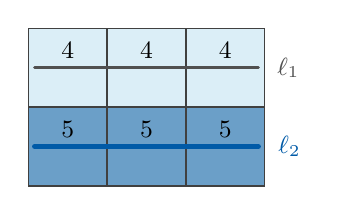
\begin{tikzpicture}[x=1.0cm,y=1.0cm]
  \raincell{0}{1}{$4$}{rainfour}
  \raincell{1}{1}{$4$}{rainfour}
  \raincell{2}{1}{$4$}{rainfour}
  \raincell{0}{0}{$5$}{rainfive!72}
  \raincell{1}{0}{$5$}{rainfive!72}
  \raincell{2}{0}{$5$}{rainfive!72}
  \drawlinks{0}
\end{tikzpicture}

% Page 2: ground-truth profile along the middle link.
\profilepanel{5}{5}{5}

% Page 3: IDW field.
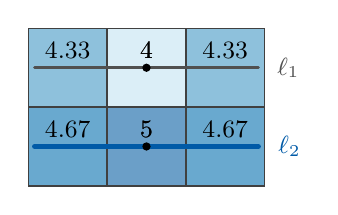
\begin{tikzpicture}[x=1.0cm,y=1.0cm]
  \raincell{0}{1}{$4.33$}{rainfourmid}
  \raincell{1}{1}{$4$}{rainfour}
  \raincell{2}{1}{$4.33$}{rainfourmid}
  \raincell{0}{0}{$4.67$}{rainfourhalf}
  \raincell{1}{0}{$5$}{rainfive!72}
  \raincell{2}{0}{$4.67$}{rainfourhalf}
  \drawlinks{1}
  % Redraw the midpoint values above the virtual-gauge markers.
  \node[font=\small] at (1.5,1.72) {$4$};
  \node[font=\small] at (1.5,0.72) {$5$};
\end{tikzpicture}

% Page 4: IDW profile along the middle link.
\profilepanel{4.6667}{5}{4.6667}

% Page 5: ILDW field.
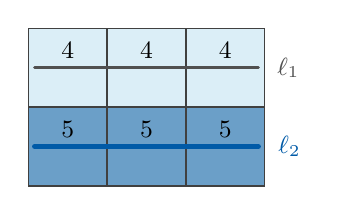
\begin{tikzpicture}[x=1.0cm,y=1.0cm]
  \raincell{0}{1}{$4$}{rainfour}
  \raincell{1}{1}{$4$}{rainfour}
  \raincell{2}{1}{$4$}{rainfour}
  \raincell{0}{0}{$5$}{rainfive!72}
  \raincell{1}{0}{$5$}{rainfive!72}
  \raincell{2}{0}{$5$}{rainfive!72}
  \drawlinks{0}
\end{tikzpicture}

% Page 6: ILDW profile along the middle link.
\profilepanel{5}{5}{5}

\end{document}
